\documentclass{scrreprt}

\usepackage{listings}
\usepackage{underscore}
\usepackage[bookmarks=true]{hyperref}
\usepackage[utf8]{inputenc}
\usepackage[english]{babel}

\hypersetup{
    bookmarks=false,    
    pdftitle={Software Requirement Specification},
    pdfauthor={Jean-Philippe Eisenbarth},                  
    pdfsubject={TeX and LaTeX},                        
    pdfkeywords={TeX, LaTeX, graphics, images}, 
    colorlinks=true,       
    linkcolor=blue,   
    citecolor=black,      
    filecolor=black,
    urlcolor=red,    
    linktoc=page    
}

\def\myversion{1.0 }
\date{}

\usepackage{hyperref}
\usepackage{graphicx}
\graphicspath{{/home/gaurabdg/Workspace/CS_F213/HotelManagementSystem/SRS_report/}}
\begin{document}
\begin{titlepage}

\begin{center}

\textup{\small {\bf CSF213 Project} \\ Report}\\[0.2in]


\Large \textbf {InnLogix\\Hotel Management System}\\[0.5in]


\normalsize Submitted by \\
\begin{table}[h]
\centering
\begin{tabular}{lr}\hline \\
ID No & Name \\ \\ \hline
\\
2016AAPS0216H & Somya Sharma \\
2016A3PS0255H & Gaurab Das Gupta \\ 
2016A3PS0272H & Utsav Kaushik\\ \\ \hline 
\end{tabular}
\end{table}

\vspace{4cm}


\includegraphics[width=0.18\textwidth]{logo}\\[0.1in]
\Large{Birla Institute of Technology and Science Pilani}\\
\normalsize
\textsc{Hyderabad Campus}
\vspace{0.2cm}\\
Second Semester 2017-18

\end{center}

\end{titlepage}

\tableofcontents


\chapter{Introduction}

\section{Purpose of the SRS}
This Hotel Management System Software Requirement Specification's (SRS) main objective is to provide a base for the foundation of the project. It gives a comprehensive view of how the system is supposed to work and what is to be expected by the end users. Client’s expectation and requirements are analyzed to produce specific unambiguous functional and non-functional requirements, so they can be used by us with clear understanding to build a system as per end user needs.

\section{Abstract}
“Hotel Management System” is a project which is developed to provide an easy and simple way for guests to communicate with the hotel administration and for the administration to manage front office capabilities such as booking reservations, guest check-in/check-out, room assignment, managing room rates, and billing to name a few. We aim to deliver a software platform that will replace time-intensive, paper and spreadsheet-heavy processes. It will also integrate other onsite services that impact the guest's complete experience, such as food and beverage operations, housekeeping and maintenance management, sales and catering, spa management.

\section{Why use InnLogix?}
Simplify reservations, improve operating efficiency and maximize revenue. 
Reduce dependency on manpower. Manual errors become a thing of the past as critical operations get automated and managed in real-time. The staff work in sync with all departments. Assign room cleaning tasks to housekeeping and track it in real-time from the frontdesk or housekeeping console. Overall it is an innovative and easy to use front desk interface that acts as a single-point dashboard to control all your operations. You can customize it to suit your hotel’s needs and manage multiple tasks at all times


\section{Overview}
The remaining sections of this documentations describes the overall descriptions which includes product perspective and functions, characteristics of users. It also consists of assumptions and constraints.




\chapter{Overall Description}

\section{Product Functions}
General functions:
\begin{itemize}
\item Customer Registration
\item Check for Availability Of Rooms
\item Payment
\item Customer Service
\item Display the Rate
\item Confirmation Of Booking
\item Set Room Details
\item Manage Booking Details
\item Generate Report
\item Email Notification

\end{itemize}

\section{User Characteristics}

There are 2 user levels in our HMS:
\begin{enumerate}
\item \textbf{Administration} is responsible for managing hotel
resources and staffs. Managers can view any information such as financial report, customer information,
booking information, and room information, analyze them and take the decision accordingly.
\item \textbf{Guest/Customers} can send requests for various services like housekeeping, lodge complaints, view their transactions.
\end{enumerate}

\section{Product Perspective}
Here's an hierarchical overview of the system: \\
\begin{figure}
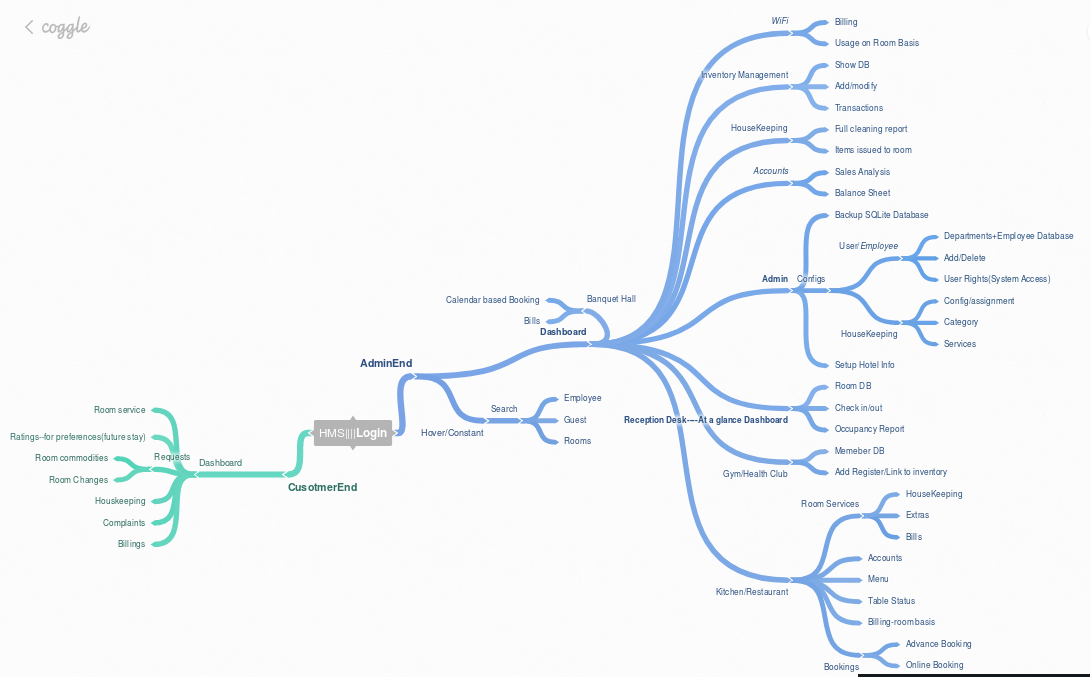
\includegraphics[scale=0.45]{mindMap}
\caption{MindMap: Click \href{https://coggle.it/diagram/Wlym2xSXOQABLTqA/t/hms-login/f320d49deb338a9cf58b394d26363a45f19cc220db5853f8cb725671b8958ee9}{here} for a better view}
\end{figure}



\section{Constraints}
Language : The system offers English only.

\section{Assumption and Dependencies}
It is assumed that system developed will work perfectly with any OS with Java SE Development Kit installed. The program will be developed with java version "1.8.0_151", 
Java(TM) SE Runtime Environment (build 1.8.0_151-b12).

The Admin side will run on desktops.
The Guest side will be a java applet accessed via intranet. But for \textbf{\textit{demo purposes}} we will showcase it as a offline jar executable file on a system.


\chapter{Specific Requirements}

\section{Software Interfaces}

Programming Language: Java

Libraries and Frameworks:
\begin{itemize}
\item JavaFX 
\item JFoenix
\item FontAwesomeFX
\item SQLite
\end{itemize}



\section{Hardware Interfaces}

Pretty basic hardware is needed to run the program.\\
User Side:
\begin{itemize}
\item Processor: AMD/Intel 1GHz
\item RAM: 512 MB
\item Disk Space: 2GB
\end{itemize}


\chapter{Functional Requiements-System Features}


\section{Login}
\begin{itemize}
\item Register an employee
\item Sign in for both guests and administration
\item “Remember me” option, so that an user need not login again and again
\end{itemize}
\begin{figure}
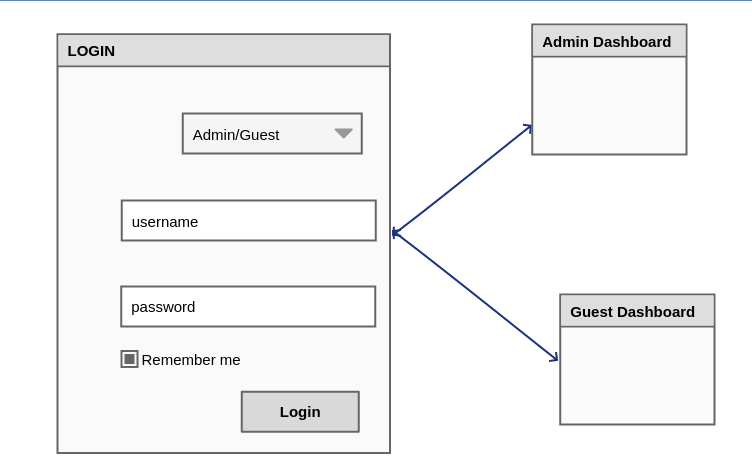
\includegraphics[scale=0.45]{login}
\caption{Login Module Data Flow}
\end{figure}


\section{Administration Dashboard}


\subsection{Admin Section}
The Admin module provides admin privileges to the head manager of your hotel to keep all the activities encapsulated from other sections, manage every modules and set access rights.
\begin{itemize}
\item Employee Database
\begin{itemize}
\item Create users, store and sort department wise
\item Set restrictions on each employee’s system access(eg. Restaurant manager can only access the kitchen section)
\item Create SuperAdmin(has privilege to access every module)
\end{itemize}
\item Setup Hotel information
\begin{itemize}
\item Link with email/OTA
\item Types of rooms with tariff
\end{itemize}
\item Front Desk Configuration
\begin{itemize}
\item Set various settings(eg, Check-in/out time late checkout charges)
\end{itemize}
\item Backup Database
\end{itemize}


\subsection{Front Office}
The Front Office module provides staff and management with an efficient tool to easily manage all front office operations within a centralized environment. Combining full guest service management with complete group billing and handling, InnLogix’s Front Office module offers seamless integration with its other modules.
\begin{itemize}
\item Room DataBase
\begin{itemize}
\item View/modify the details of the rooms available
\item Add new rooms under various categories
\end{itemize}
\item Guest check-in
\begin{itemize}
\item Registration form with payment options
\item Upload identity proof pdf
\item Search existing guest database with name/mobile number
\end{itemize}
\item Guest check-out
\begin{itemize}
\item Get total bill of charges(meals, spa etc.) incurred during the whole stay on one-click
\item Print the receipt
\end{itemize}
\item Main Dashboard
\begin{itemize}
    \item At a glance color coded view of all the rooms’ status
    \item Click on a “card” to see all the corresponding details(guest’s details, maintenance status etc)
    \item Access services from the card. This will be the admin side view of all the requests/complaints(room change) the guest has made through the customer end through this application.
    \item Get occupancy report
\end{itemize}
\end{itemize}

\subsection{Housekeeping}
The Housekeeping module of InnLogix enables the user to enter and track information that is required to manage the hotel’s housekeeping, with instant updating of room status.
\begin{itemize}
    \item Get cleaning report of all the rooms given by floor superintendent with log, timestamp etc.
    \item Keep a check on items issued to room
\end{itemize}

\subsection{Kitchen/Restaurant}
The Restaurant module is a one stop solution for managing your restaurant with table reservations, ordering, accounts all in one place.
\begin{itemize}
    \item Managing food menu and keep a check on availability of  items
    \item Guests can login to this portal and place their order for room service
    \item Generating a bill for all the deliveries to a particular guest user
    \item Table Occupancy Status
\end{itemize}

\subsection{Spa/Gym}
Manage the facilities provided by the hotel.
\begin{itemize}
    \item Getting the membership for the Gym or Spa
    \item Keep a check of available timings
\end{itemize}

\subsection{Bookings}
Manage the booking aspects of your hotel.
\begin{itemize}
    \item Keeping the record of already booked rooms-available for online hotel booking websites
    \item Online Booking
\begin{itemize}
    \item Advance Booking Discount
    \item Seasonal Room Tariff
    \item Booking date blocking
    \item Default Bank Account 
\end{itemize}
\end{itemize}

\subsection{Banquet Hall}
Manage your banquet hall's bookings and maintenance.
\begin{itemize}
\item Manage bookings based on availability through a calendar based system
\item Get reports on transactions , stock etc.
\end{itemize}

\subsection{Inventory Management}
Keep track of all your inventories and analyse your deals.
\begin{itemize}
\item Get list of purchased items centre wise like “Kitchen Stock” etc.
\item Modify the item list
\item Keep track of the transactions made with suppliers
\end{itemize}

\subsection{Accounts Panel}
All your accounts in one place supplying you with all the analytics.
\begin{itemize}
    \item Complete Management of Accounting :
\begin{itemize}
    \item Profit and Loss
    \item Balance Sheet
    \item Account Statement
    \item Daily Statistics Report
\end{itemize}
\end{itemize}

\section{Guest Dashboard}
InnLogix’s Guest Interface module provides the features you need to support the needs of your members. From member billing and statements to expense tracking, this module will help you gain control of your member accounting.

\subsection{Requests}
The guest can forward their requests to the administration through this module.
\begin{itemize}
\item Various commodities
\item Room change
\item Extra bed
\end{itemize}
\begin{figure}
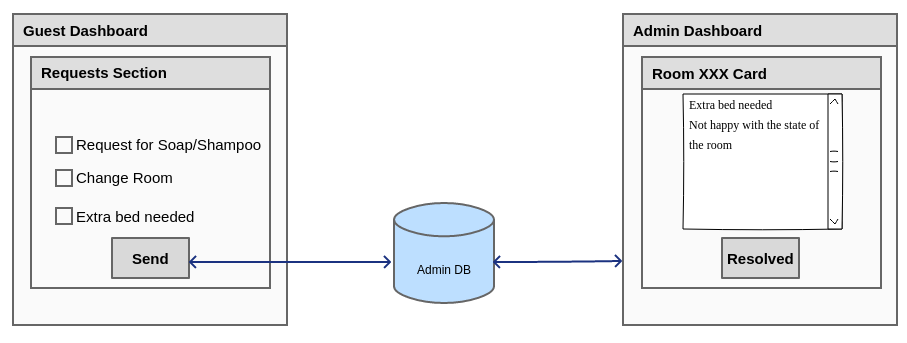
\includegraphics[scale=0.45]{requests}
\caption{Requests Module Data Flow}
\end{figure}

\subsection{Housekeeping}
The guest can avail housekeeping services and specify their needs through this.
\begin{itemize}
    \item Guest can set the timings when the room will be free
    \item Complaints
\end{itemize}
\begin{figure}
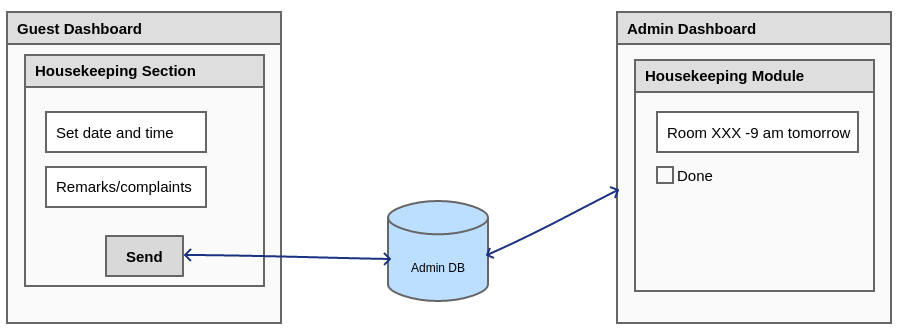
\includegraphics[scale=0.45]{housekeeping}
\caption{Housekeeping Module Data Flow}
\end{figure}

\subsection{Room Service}
Guests can avail room service from anywhere-for example they can pre-order meals even if they are not present in the hotel.
\begin{itemize}
\item Request for room service for various reasons, all linked to the admin side
\end{itemize}
\begin{figure}
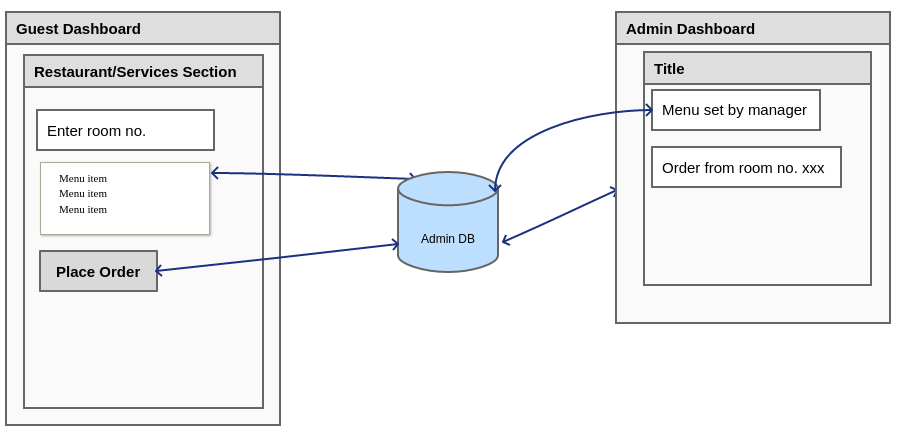
\includegraphics[scale=0.45]{food}
\caption{Services/Restaurant Module Data Flow}
\end{figure}

\subsection{Complaints}
All the lodged complaints through this module will be sent to the administration.
\begin{itemize}
    \item Guests can lodge complaints to various departments
    \item They can also give ratings and preferences such that you know them well and offer a more pleasant stay the next time they visit
\end{itemize}
\begin{figure}
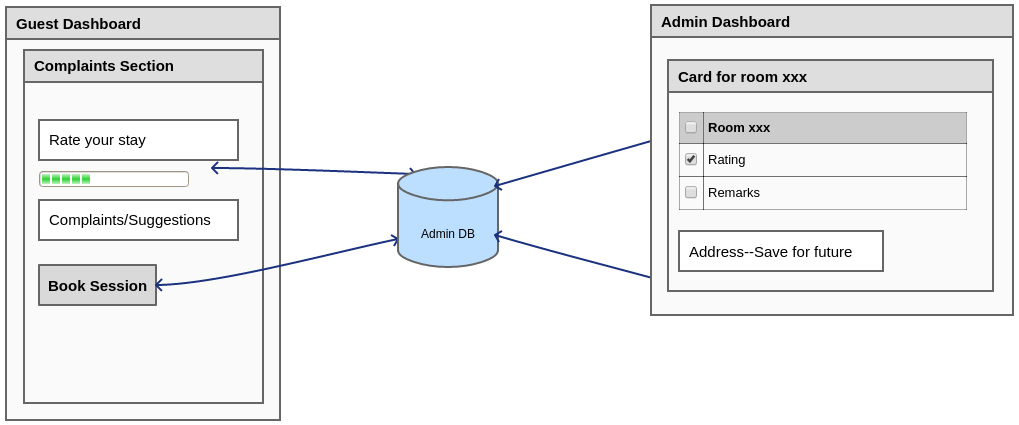
\includegraphics[scale=0.45]{ratings}
\caption{Complaints/Ratings Module Data Flow}
\end{figure}

\subsection{Billings}
All of the guest's transaction, in one place.
\begin{itemize}
    \item Send all the transactions(gym/spa/restaurant/laundry) that take place daily
\end{itemize}
\begin{figure}
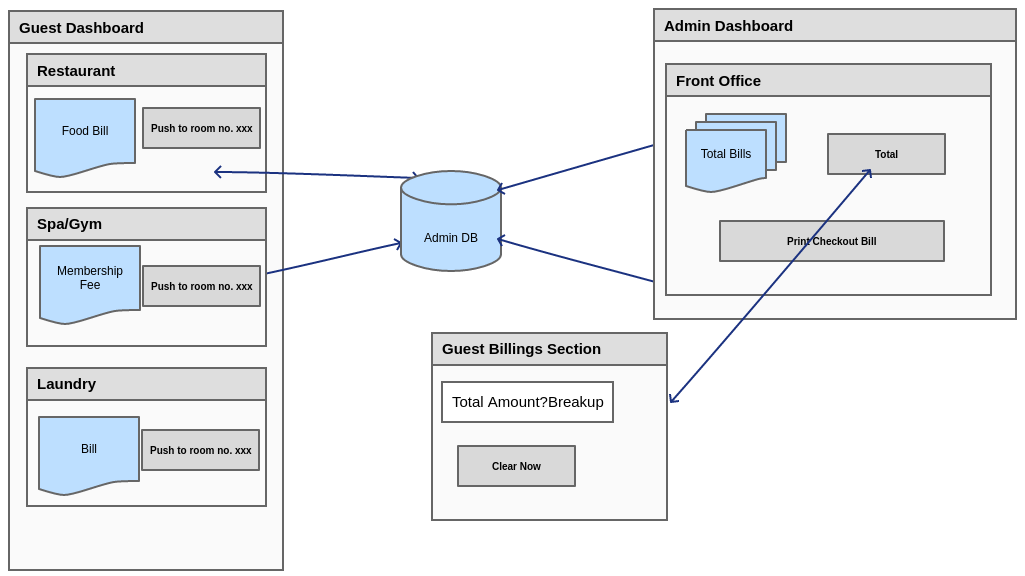
\includegraphics[scale=0.45]{bills}
\caption{Billings Module Data Flow}
\end{figure}

\subsection{Services}
Miscellaneous Services can be availed through this.
\begin{itemize}
    \item Placing the time slot for your gym/spa session
    \item Placing order from outside
    \item Reservation table
\end{itemize}
\begin{figure}
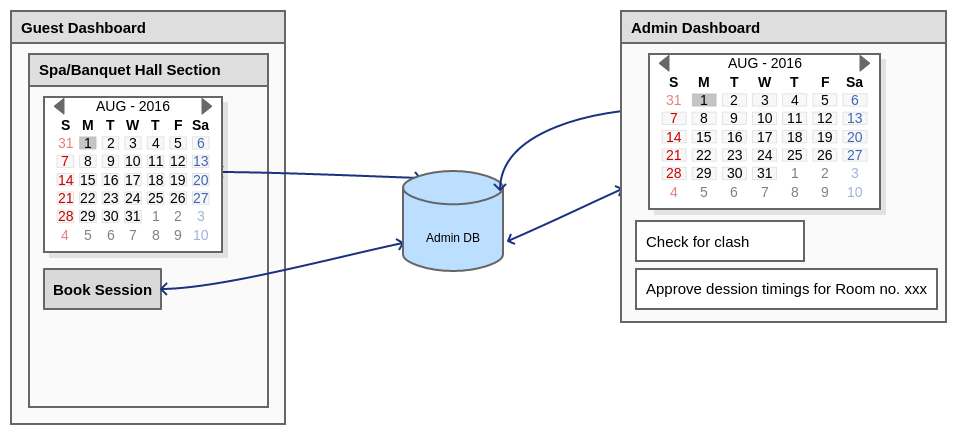
\includegraphics[scale=0.45]{spa}
\caption{Services Module Data Flow}
\end{figure}

\subsection{WiFi Usage}
\begin{itemize}
    \item It will show the guest how much data he/she has used
    \item Option to pay for extra data
\end{itemize}


\chapter{Nonfunctional Requirements}

\section{Performance Requirements}
Performance should not be an issue because all of our queries involve small pieces of
data. Changing screens will require very little computation and thus will occur very quickly.
These functions will be optimized to make it highly efficient:
\begin{itemize}
    \item Data update in database 
    \item Queries returning results 
    \item Load time of UI 
    \item Login Validation 
    \item Response to customer inquiry 
    \item Report should be generated automatically every day for manager and anytime upon request
\end{itemize}

\section{Security Requirements}
All data must be stored, protected or protectively marked.

\section{Safety Requirements}
\begin{itemize}
    \item Database should be backed up every hour
    \item Under failure, system should be able to come back at normal operation under an hour
\end{itemize}

\section{Capacity Requirements}
\begin{itemize}
    \item Not more than 20,000 members to be registered
    \item System need to handle at least 30 transactions during peak hours
\end{itemize}

\end{document}
